
\subsection{Основы квантово-механической теории строения атома в контексте образования химической связи.}

 В соответствии с волновой механикой, какая-либо микросистема
описывается функцией состояния, или волновой функцией, которая
является функцией координат всех частиц, образующих эту систему
и от времени, если эта система находится не в стационарном
состоянии. Вероятность нахождения частицы в бесконечно малом
объёме пропорциональна квадрату $\psi^2$ ее волновой функции или
произведению $\psi\cdot\psi$, где $\psi*$ - комплексно-сопряженная $\psi$, если
волновая функция - комплексная величина. Как и другие волны,
волновая функция имеет области положительных и отрицательных
амплитуд, но знак не имеет физического смысла, если в одной
области пространства есть только одна волновая функция. Если же
их две, знак волновой функции имеет чрезвычайно важное
значение.

В результате их интерференции аплитуда
результирующей волновой функции может либо повыситься, если
исходные волновые функции имели одинаковые знаки в данной
области, либо понизиться, если волновые функции имеют
противоположные значения.

Термин «химическая связь» не имеет строгого определения. Для
ковалентных соединений с позиций квантовой механики это есть
результат взаимодействия нескольких волновых функций. Согласно
методу валентных связей, волновая функция электронной пары
формируется путем наложения волновых функций для отдельных
фрагментов молекулы, то есть является суперпозицией волновых
функций каждой конфигурации. Образование связи можно
представить как высокую вероятность нахождения двух электронов
между двумя ядрами. Например, связь в молекуле водорода
описывается следующим образом. Были выбраны орбитали
каждого атома с одним электроном $(\psi(A)$ и $\psi(B))$, и
соответствующие волновые функции объединяют в волновую
функцию одновременно двух электронов.

$$\psi = \psi_A(1)\cdot\psi_B(2) + \psi_B(1)\cdot\psi_A(2)$$

Эту операцию называют спариванием электронов, что является процессом с проигрышем энергии.

С позиции метода молекулярных орбиталей, движущей силой образования ковалентной связи является делокализации электронов. Одноэлектронные функции - молкулярные орбитали, каждую из которых можно рассмотреть как линейную комбинацию атомных орбиталей -- сумму атомных орбиталей с различными коэффициентами. Пример для $H_2$:

$$\psi = C_A\varphi_A + C_B\varphi_B$$

$$1) C_A =  CB= 1;  \psi_+ = \varphi_A + \varphi_B$$

Связывающая орбиталь. Связывающий характер объясняется интерференцией двух атомных орбиталей с одинаковыми по знаку амплитудами, что является причиной повышения амплитуды волновой функции между ядрами. Электрон, занимающий эту орбиталь, с повышенной вероятностью находится в межъядерном пространстве и может сильнее взаимодействовать с обоими ядрами.

$$C_A =1; C_B = -1; \psi_- = \varphi_A-\varphi_B$$

Разрыхляющая орбиталь. Большая энергия электрона на этой орбитали
возникает вследствие интерференции двух атомных орбиталей с разными по
знаку амплитудами, при этом амплитуды волновых функций вычитаются и
между двумя ядрами образуется узловая плоскость.

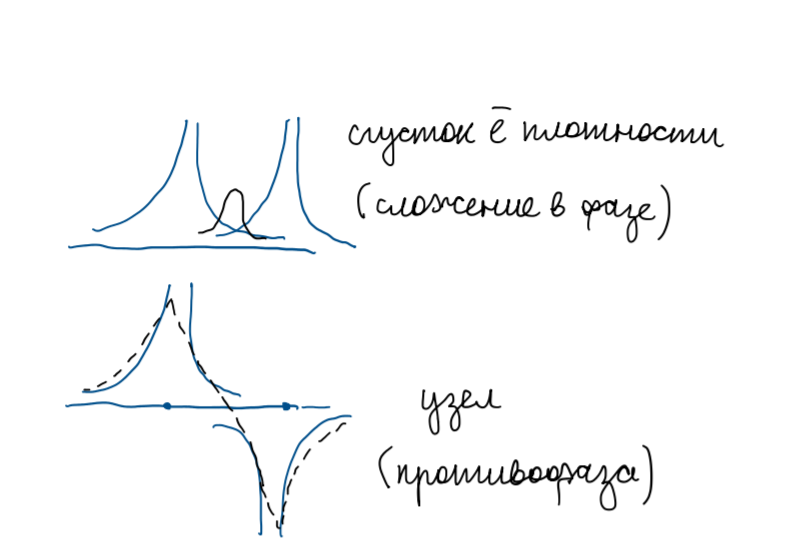
\includegraphics[scale=0.7]{images/1v.png}
